\subsection{Data Visualization Research}
With the field of soundscape ecology being a relatively new one, the format of data visualizations is not yet cemented in the community. In addition to the basic functionality of our service, another goal of this project is to research and define useful visualizations for both researchers and data consumers. Each index analyzes a different thing in nature, so not all forms of data representations will apply. The goal of this section is to shed light on the reasoning behind the decisions to use each index\textquotesingle s respective visualization in the service.

\subsubsection{Outlier Identification}
An important part of the analysis of the sound files is to identify when outliers arise. Our sponsor has expressed that being able to see when an outlier occurs and being able to listen to what caused it is important in drawing conclusions and finding interesting bits of information from a data set. Thus, two infographics seem reasonable, those being timelines and line charts. Both do relatively similar jobs, however a timeline is made specifically for information over time. The only upside to a line graph would be that each point on the graph would represent a sound file, and the results of its analysis. Being able to represent an output as a small dot on a chart and allowing the user to select or hover over that point to see which file caused the outlier is certainly desirable from a usability perspective. Implementing a full-fledged sound file analysis section seems a bit out of scope for this project, so a line graph used to represent each sound file in a data set and the results of each file\textquotesingle s analysis is the best way to help the user identify outliers in the data.\par

\begin{center}
  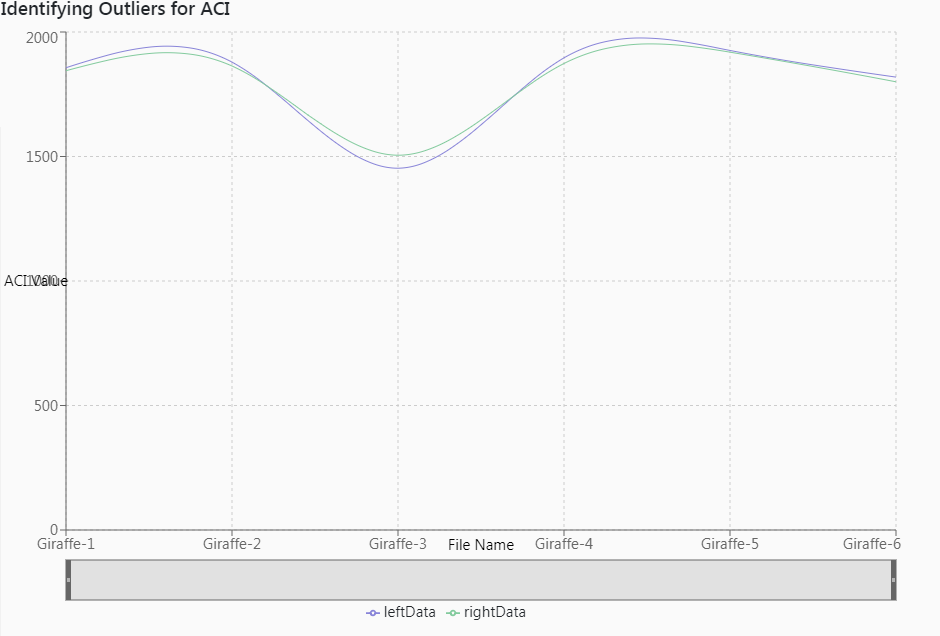
\includegraphics[width=\textwidth]{OutlierACIgraph1} \\[12pt]
  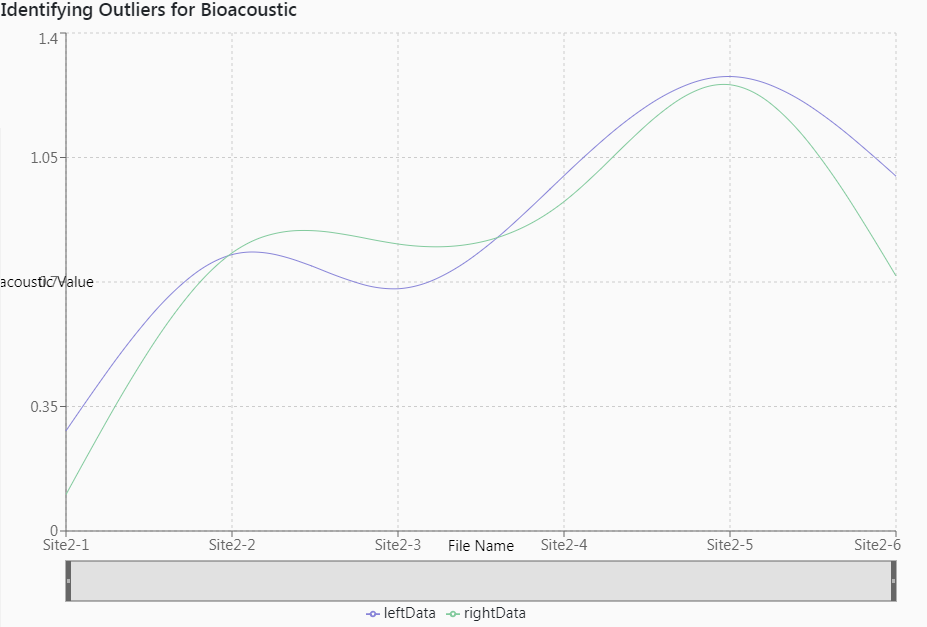
\includegraphics[width=\textwidth]{OutlierBAgraph1} \\[12pt]
\end{center}
The graphs above are for a data set comprised of files that the ACI and Bioacoustic Index was run on. The X axis displays the file name, while the Y axis labels the respective index value. Notice that file Giraffe 3 is much lower than the rest in the first graphic, and the file Site2-1 and Site2-5 also stand out in the second. Using these visuals, a researcher can quickly identify which files in their sets contain possibly interesting sounds to listen to in order to make further conclusions about their data.

\subsubsection{NDSI Visualization}
The NDSI index measures the relationship between biophony and anthrophony at a site. This is elaborated on in the Overview of Indices section of this report. Because the NDSI is used for comparing two different variables, the representation for this index is different from that of ACI or ADI. Here, two bar charts have been chosen, one for comparing the values per channel, and one for comparing the values side by side.\\

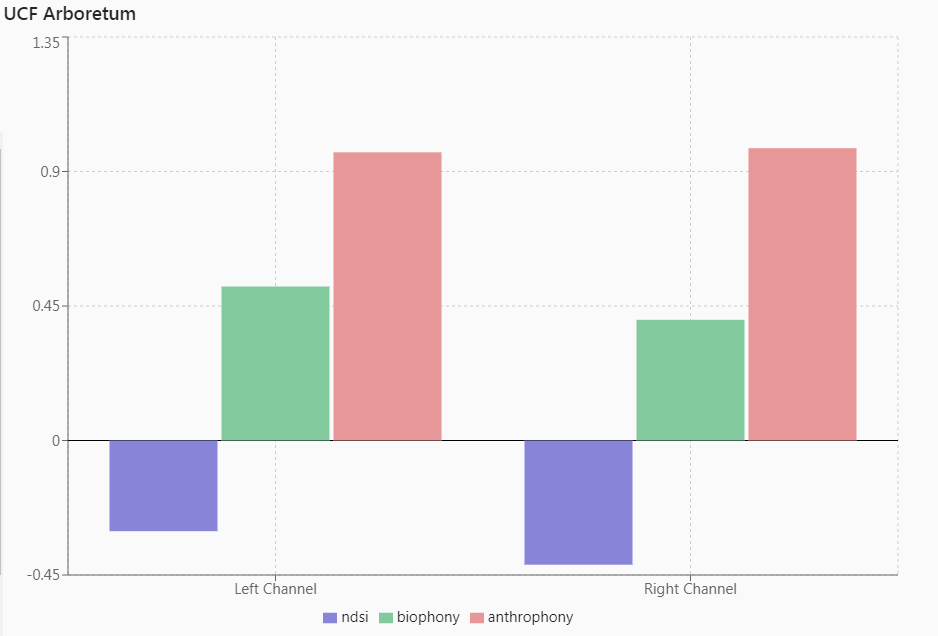
\includegraphics[width=\textwidth]{NDSIgraph1}
The first visualization available is a bar graph comparing the two channels. Each channel has an overall NDSI value, along with biophony and anthrophony values. Because the NDSI is a difference of the anthrophony and biophony, it is useful to view them side by side like so. The user is also able to hover over any bar and see the respective data values as they please.\\

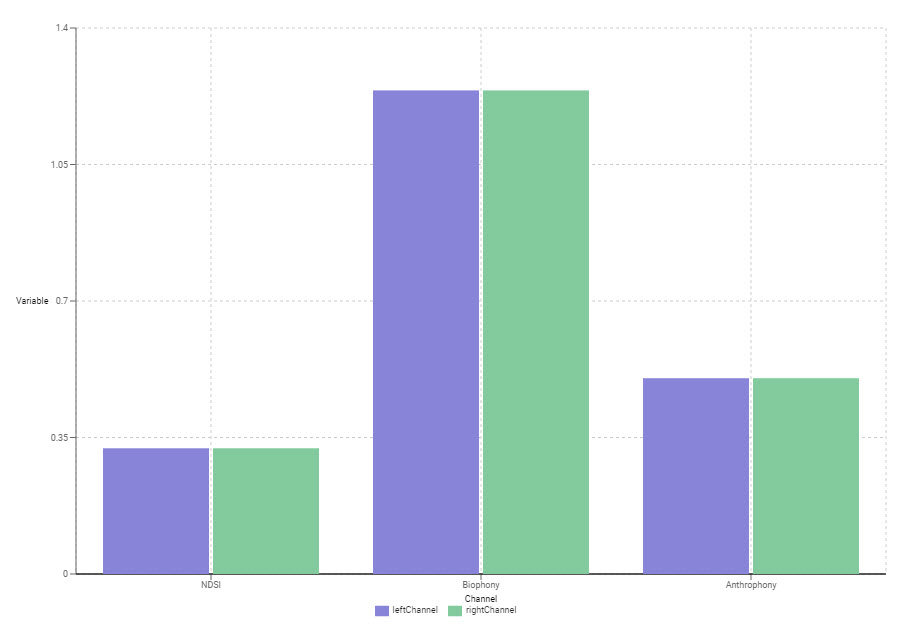
\includegraphics[width=\textwidth]{NDSIgraph2}
The other visualization available is another bar graph, this one showing the NDSI values, anthrophony values, and biophony values side by side, sorted by channel this time. This representation is useful because sometimes one channel of the microphone gets different data outliers than the other, so being able to identify which channel has these outliers is helpful for research.

\subsubsection{ACI Visualization}
As ACI is best represented over a period of time, the first infographics that come to mind for representing it are line charts and histograms. A line chart would be able to represent ACI values over time and also represent multiple results across time. This benefits users because it allows them to visually compare results taken at the same time of day, but from different days. Our sponsor mentioned that being able to see if there is a correlation between time of day and when a site is loud or quiet is useful in research. A histogram on the other hand is best fit for representing the distribution of a single variable over time. This would be useful for representing a single result, instead of comparing results over time. Thus, the two visualizations initially available for ACI were line charts for comparing results, and a histogram for individual results.\\

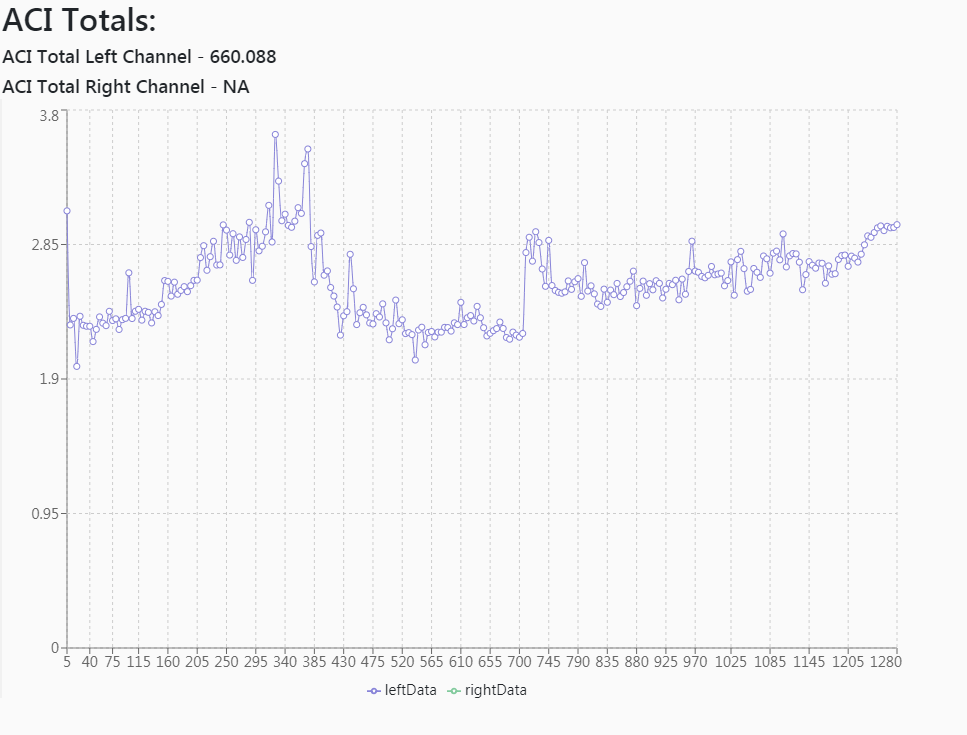
\includegraphics[width=\textwidth]{ACIgraph1}
This was the first idea for creating a visualization of ACI. This graph included the ability to see the specific value for each data point, which is useful for researchers. The X axis represents the time stamp in the file, and the Y axis represents the ACI value at that time stamp. The heading of the graph includes the ACI total value for both the left and the right channel. This graph is nice, however it does not include the ability to zoom into a specific time range, something that can be useful especially for longer files. Thus the next iteration came to fruition.\\

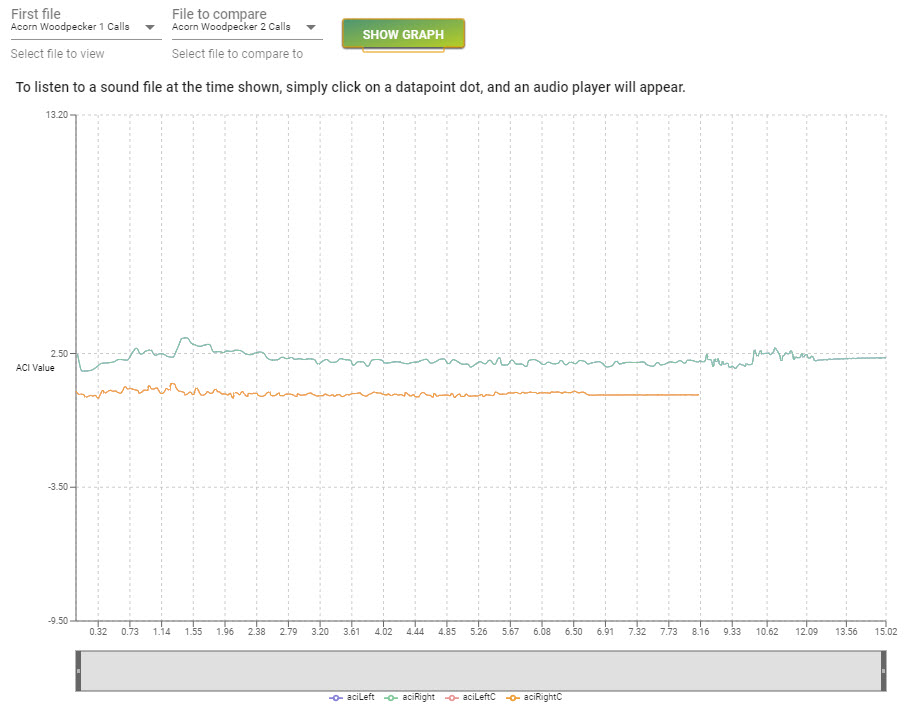
\includegraphics[width=\textwidth]{ACIgraph2}
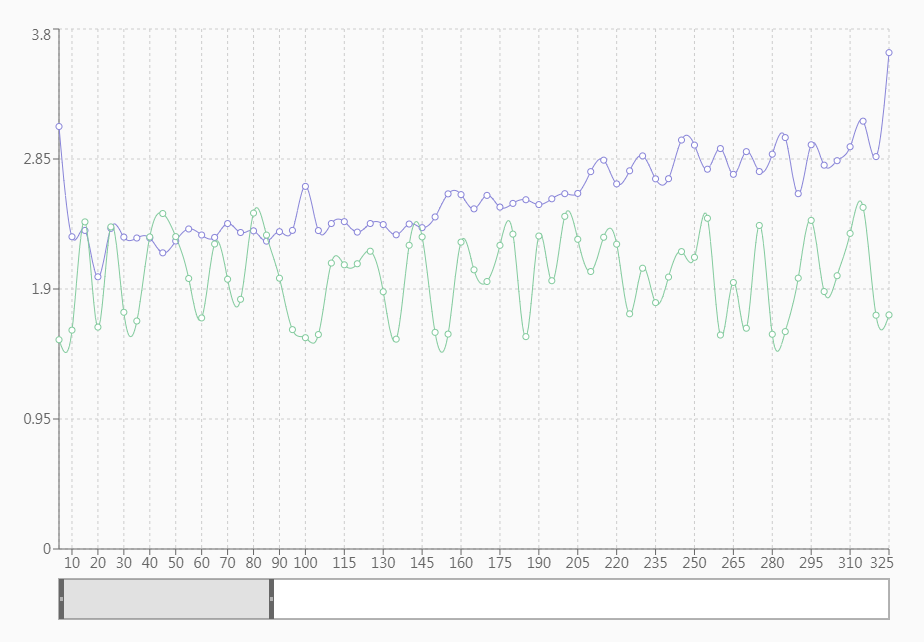
\includegraphics[width=\textwidth]{ACIgraph2-1}
These graphs are similar to the first version, however they include a brush bar. This bar can be used to specify a range of time that the graph natively zooms in on, as shown in the second image. In addition, that range of time can be scrolled through, so the user could filter by thirty second intervals and manually scroll through the data as they please. We feel this visualization is the best representation for both the data and the user.\\

\subsubsection{ADI and AEI Visualization}
The ADI and AEI indices measure the diversity and evenness of sounds in a sound file, usually used to draw conclusions as to the diversity of animals at the site. For these indices, a single value is used to represent their values. The algorithms used in this service provide both a right and left channel ADI and AEI value where relevant, along with band values for each frequency range tested. Thus, a single numerical value representation for single file or dataset analysis is available, along with a graph showing these values at each band range. However for comparing ADI and AEI across data sets, it may be more beneficial to use these single values to create a line graph. See the comparison section for more details on this. In addition, it is useful to compare the ADI and AEI, and when the user does \textit{both} indices on a file or data set, the service will compare them appropriately using a line graph.\\

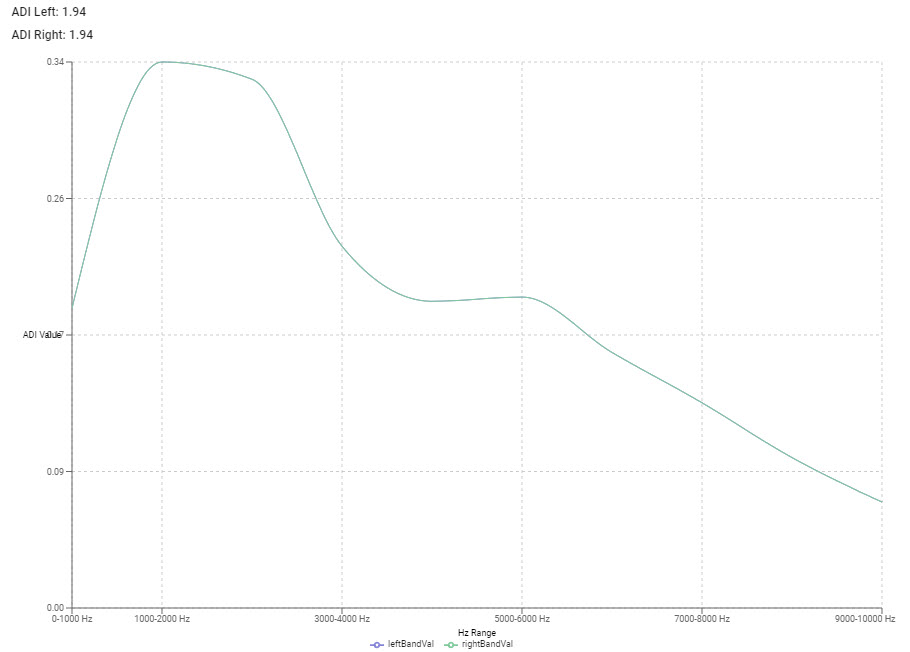
\includegraphics[width=\textwidth]{ADIgraph1}
This visualization is done on a single file using the ADI index. The X axis shows the band ranges that were determined by the user, while the Y axis shows the ADI values. This line chart also includes the ability to hover over data points to see the exact data. In addition, reference lines have been added to show the ADI value for the right and left channels, to show the average values as a baseline.

\subsubsection{Bioacoustic Index Visualization}
For the Bioacoustic index, the value output by the algorithms is an area value under a curve for both the left and right channels where relevant. Thus initially, the best representation of this index would be a stacked area graph, with both the left and right channels included.\\

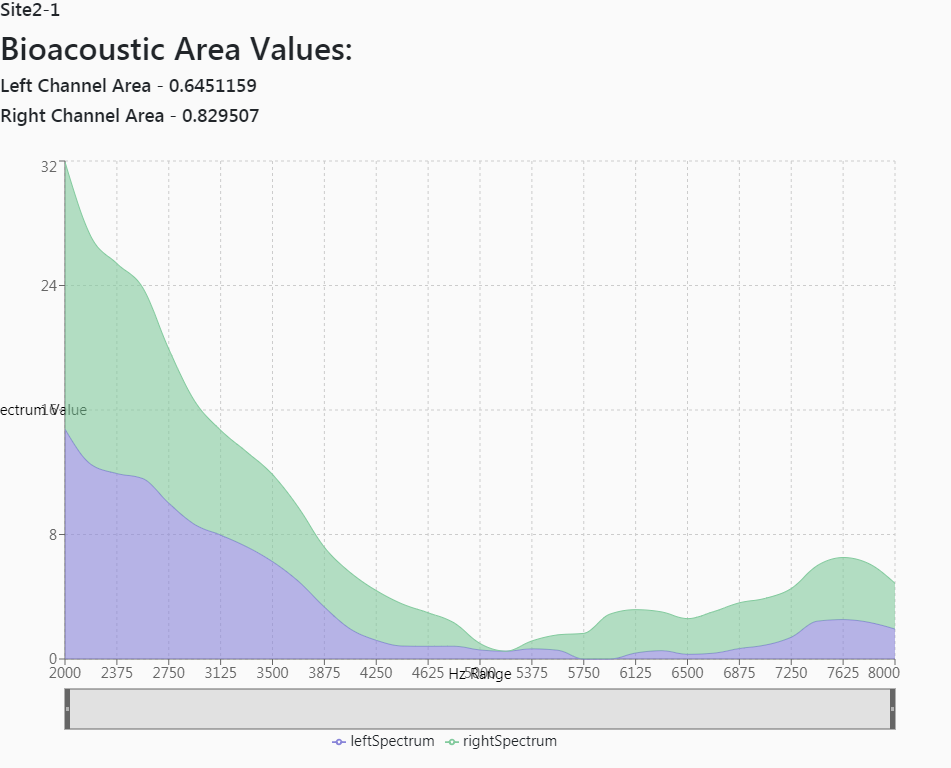
\includegraphics[width=\textwidth]{BAgraph1}
This graph includes both channels, with a brush included much like in ACI. Because the index calculates a literal area under a curve, an area chart is logically the best representation, and the graphic helps to support this. Again, the user can filter by hertz range using the brush, giving insight into the values in specific ranges. Upon further testing though, it turned out that this particular stacked area graph was not a good way to represent the channels, as their values were not dependent on each other. Thus the following graphs were finalized.\\

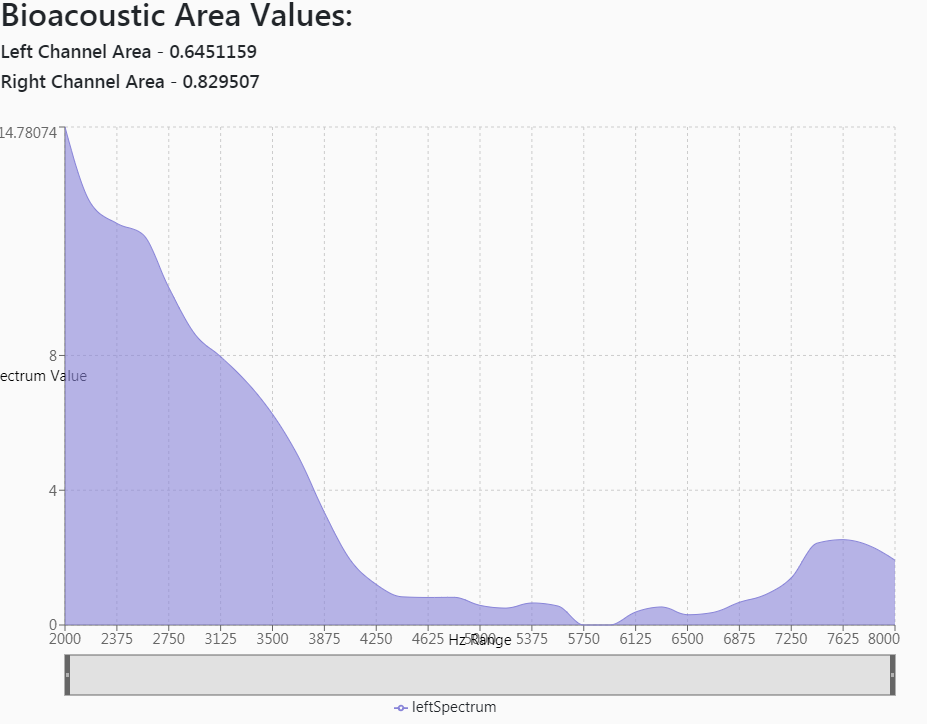
\includegraphics[width=\textwidth]{BAgraph2-1}
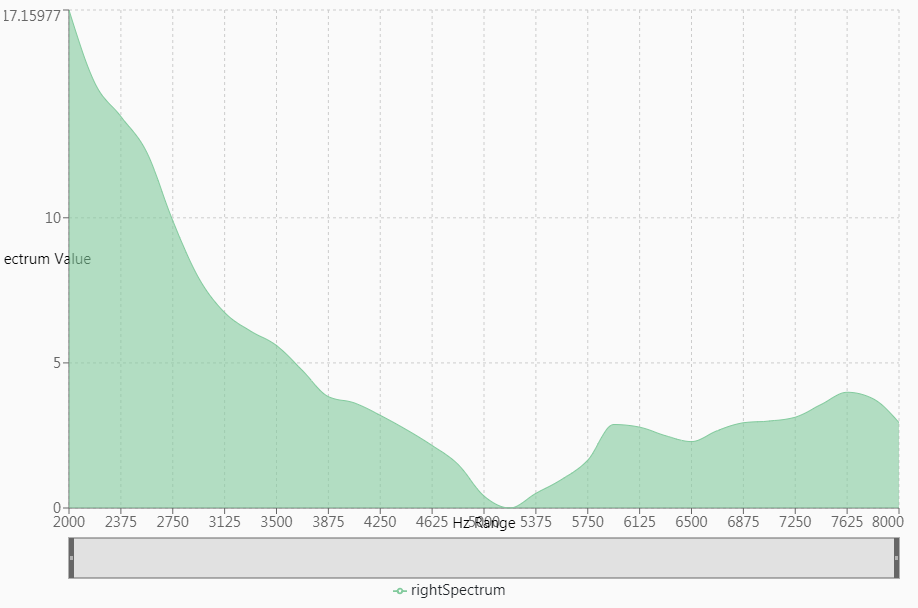
\includegraphics[width=\textwidth]{BAgraph2-2}
These are a much better representation of the channel areas, as they are no longer dependent on eachother as in the last iteration.

\subsubsection{Comparing Data Sets and Files}
Comparing data sets is maybe the most important feature of this service. In doing this, a researcher can evaluate index values over time, using different data sets for different things. For example, a researcher may be working in a site, recording data in the morning and at night, every day for a week. The researcher would process both sets separately using whichever indices and parameters they wish, and name and tag the sets appropriately. Then, in the Catalog, they can select both data sets, and see visualizations comparing the two sets across time, to see how the index values match up on the same days but in the morning and at night.\par
From a research perspective, this is the best way to draw conclusions from the indices included in this service, as the more data that is collected and processed, the more sense they make. An example of this includes a forest where human interaction is on the rise. Using an index like ACI over time will help to make correlations as to how human invasion on the forest is affecting the wildlife. Alternatively, for comparing across sites, if a species of animal is found in multiple locations, the ACI index can be used to roughly determine the number of these species in the area. Comparing this value across the sites is useful for determining species population in different areas.\\

\begin{center}
	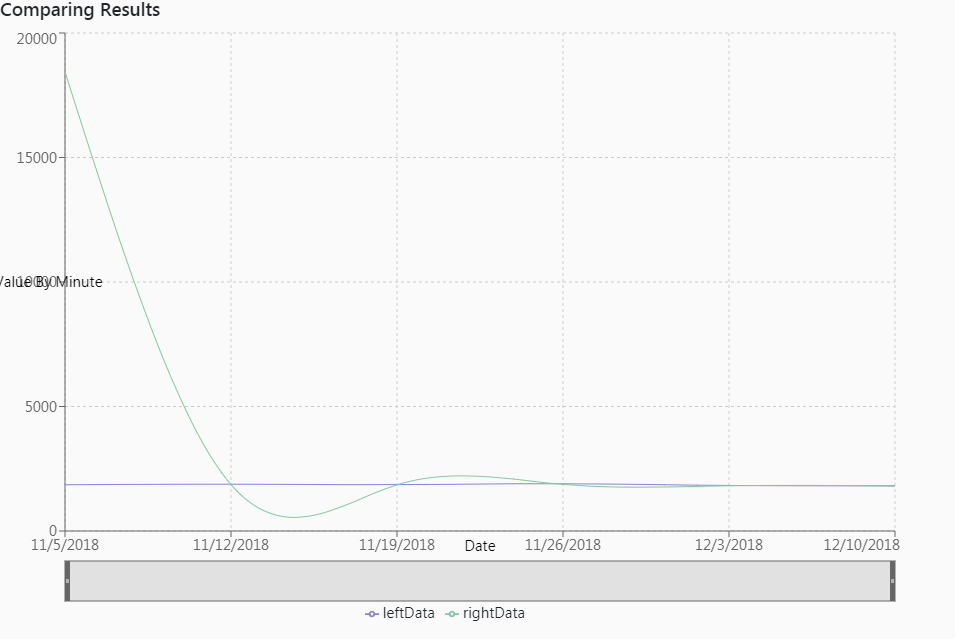
\includegraphics[width=\textwidth]{CompareACIgraph1} \\[12pt]
	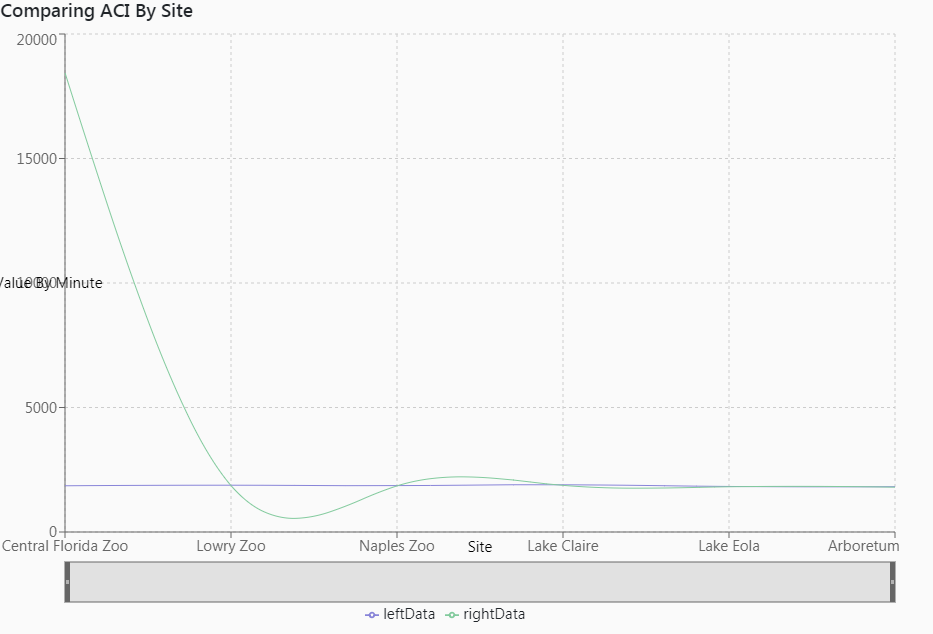
\includegraphics[width=\textwidth]{CompareACIgraph2} \\[12pt]
\end{center}

The first is a comparison graphic for ACI index across time. The data used was six files, all recorded a week apart. The X axis represents the date of each file, and the Y axis shows the ACI value by minute for each date. The other comparison available for ACI is comparing across data sites. Much like the other ACI comparison graph, the Y axis again shows the ACI value by minute, while the X axis for this graph represents the site. Overall, these two comparison charts give the researcher two different comparison insights for the ACI index.\\

\begin{center}
	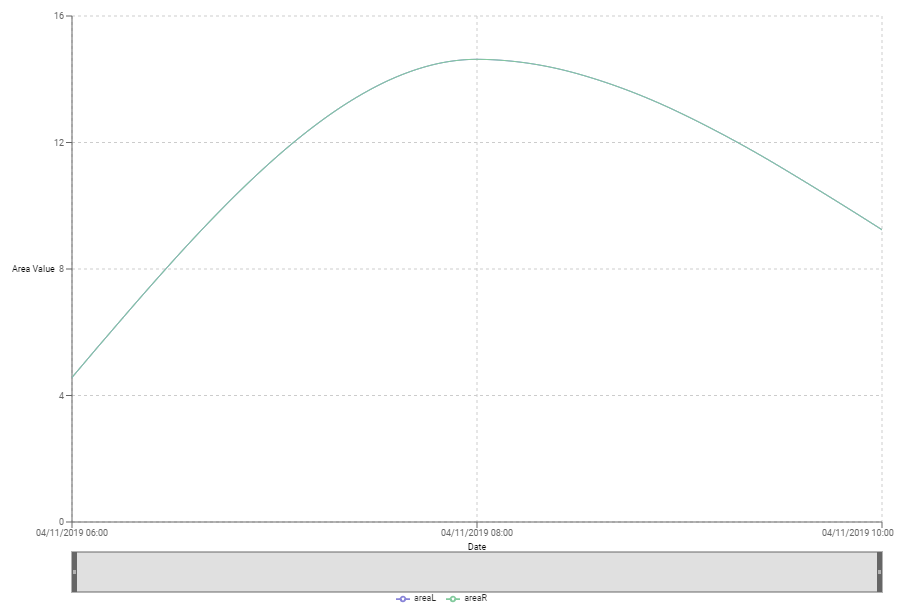
\includegraphics[width=\textwidth]{CompareBAgraph1} \\[12pt]
	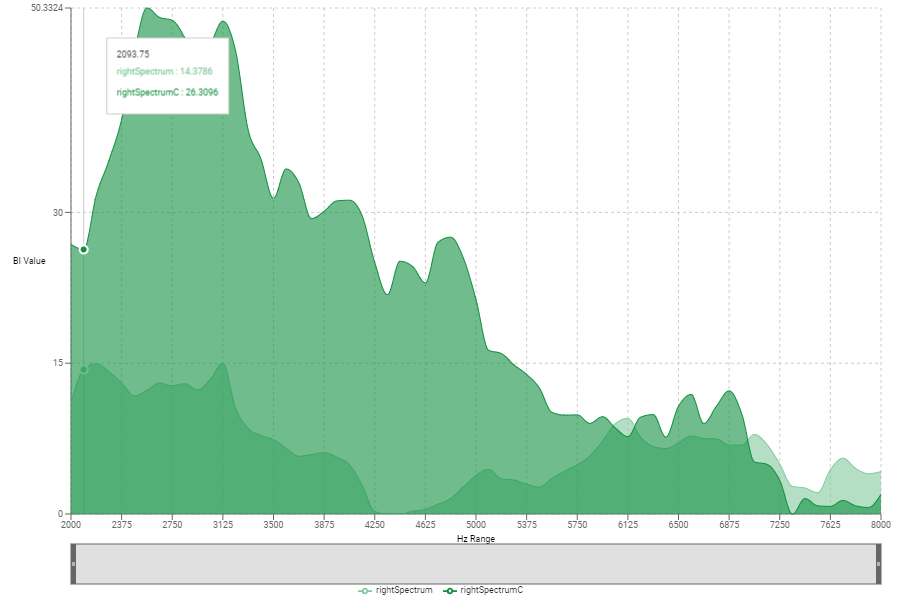
\includegraphics[width=\textwidth]{CompareBAgraph2} \\[12pt]
\end{center}

These two graphs represent the comparison charts available for the Bioacoustic Index. Again, the user has comparison across dates and research sites available to them. The brush is included to allow the user to shorten the observed time range as they please.\\

\begin{center}
	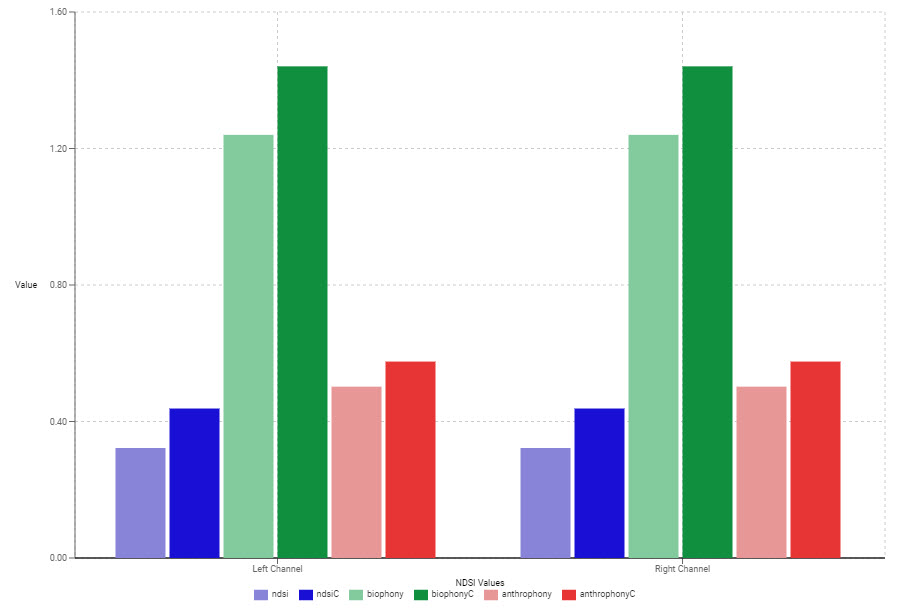
\includegraphics[width=\textwidth]{CompareNDSIgraph1} \\[12pt]
	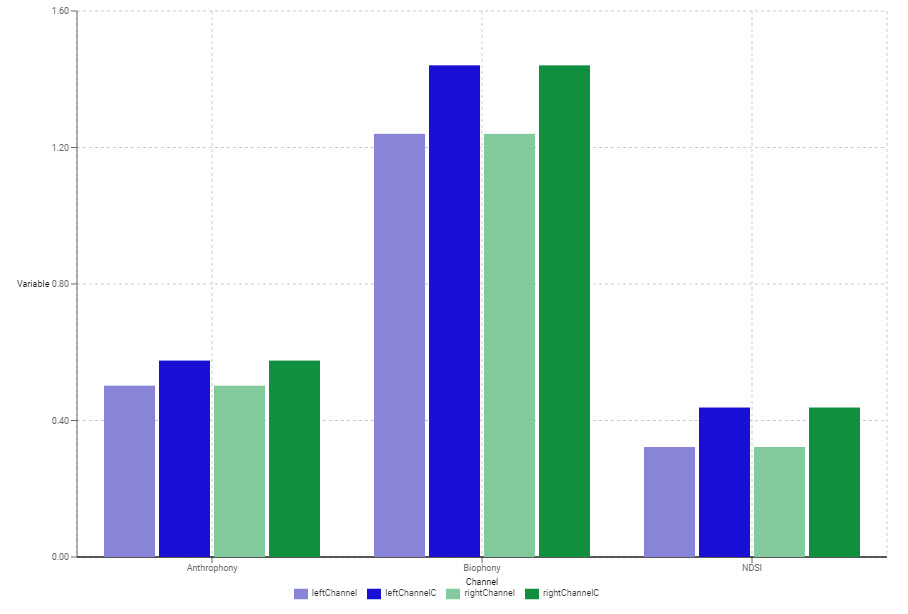
\includegraphics[width=\textwidth]{CompareNDSIgraph2} \\[12pt]
\end{center}

The NDSI index includes three different variables of interest to the user. These two images show the biophony comparison across date and the NDSI comparison across sites respectively. These charts are bar graphs to show the respective value by channel, along with a line that helps to show the change intensity between values. Notice that the NDSI is upside down, this is because NDSI values are typically negative due to the nature of the index. A brush is included as per usual.\\

\begin{center}
	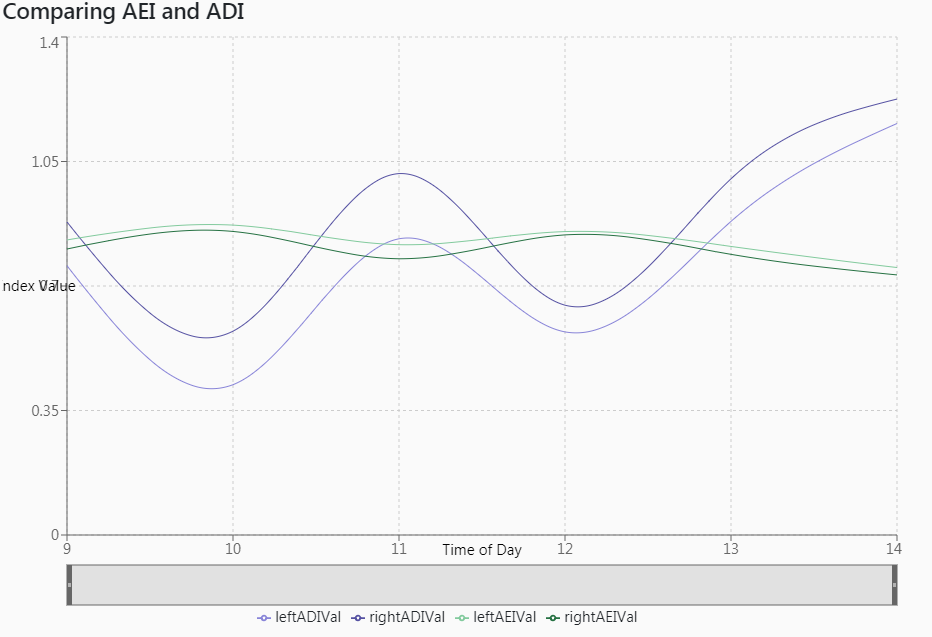
\includegraphics[width=\textwidth]{ADIAEIgraph1} \\[12pt]
\end{center}
ADI and AEI indices are closely related, thus it is useful for the user to be able to view them side by side. In the graphs available, as long as a data set has had both ADI and AEI run on it, the user will have the option to view the AEI and ADI data individually, as shown in their respective section, but also side by side, as seen above. This graph shows the ADI and AEI values for each channel over the time of day they were recorded. They are color coded to show their relationship to one another by channel, and contrast each other by index. A brush is also included.

